\section{Рабочий проект}
\subsection{Классы, используемые при разработке}

В процессе разработки программной информационной системы были использованы различные классы, каждый из которых выполняет строго определённую функцию в архитектуре приложения. В таблице \ref{class:table} приведён перечень ключевых классов, описание их назначения, модули, в которых они реализованы, а также перечень основных методов. Такая структура помогает обеспечить модульность, читаемость и масштабируемость системы.

\renewcommand{\arraystretch}{0.8} % уменьшение расстояний до сетки таблицы
\begin{xltabular}{\textwidth}{|X|p{2.5cm}|>{\setlength{\baselineskip}{0.7\baselineskip}}p{4.85cm}|>{\setlength{\baselineskip}{0.7\baselineskip}}p{4.85cm}|}
	\caption{Описание классов, используемых в приложении\label{class:table}}\\
	\hline \centrow \setlength{\baselineskip}{0.7\baselineskip} Название класса & \centrow \setlength{\baselineskip}{0.7\baselineskip} Модуль, к которому относится класс & \centrow Описание класса & \centrow Методы \\
	\hline \centrow 1 & \centrow 2 & \centrow 3 & \centrow 4\\ \hline
	\endfirsthead
	\caption*{Продолжение таблицы \ref{class:table}}\\
	\hline \centrow 1 & \centrow 2 & \centrow 3 & \centrow 4\\ \hline
	\finishhead
	NormalMap\allowbreak App & main.py & Главный класс графического интерфейса. Управляет загрузкой изображения, генерацией нормалей, запуском визуализации и отображением результата. & load\_image(), generate\_normal\_map(), visualize(), save\_output()\\
	\hline GLCube\allowbreak Widget & glcube.py & OpenGL -- виджет для визуализации карты нормалей в 3D-режиме. Отвечает за отображение куба и освещения. & initializeGL(), paintGL(), resizeGL()
\end{xltabular}
\renewcommand{\arraystretch}{1.0} % восстановление сетки

\subsection{Функции программной системы}

Программная система состоит из набора функций, каждая из которых отвечает за конкретную задачу в рамках обработки изображений, генерации карт нормалей или визуализации результата. Таблица \ref{func:table} содержит список основных функций, описание их назначения и указание на модули, где они применяются.

\renewcommand{\arraystretch}{0.8} % уменьшение расстояний до сетки таблицы
\begin{xltabular}{\textwidth}{|p{4.85cm}|>{\setlength{\baselineskip}{0.7\baselineskip}}p{2.5cm}|X|>{\setlength{\baselineskip}{0.7\baselineskip}}p{4.85cm}|}
	\caption{Описание функций, используемых в приложении\label{func:table}}\\
	\hline \centrow \setlength{\baselineskip}{0.7\baselineskip} Название функции & \centrow \setlength{\baselineskip}{0.7\baselineskip} Модуль, к которому относится функция & \centrow Назначение \\
	\hline \centrow 1 & \centrow 2 & \centrow 3\\ \hline
	\endfirsthead
	\caption*{Продолжение таблицы \ref{func:table}}\\
	\hline \centrow 1 & \centrow 2 & \centrow 3\\ \hline
	\finishhead
	\_\_init\_\_(self) & ui.py & Конструктор главного окна. Инициализирует интерфейс и параметры.\\
	\hline update\_strength(self, value) & ui.py & Обновляет значение силы градиента по слайдеру. \\
	\hline update\_depth(self, value) & ui.py & Обновляет параметр глубины нормалей. \\
	\hline update\_operator(self, text) & ui.py & Устанавливает выбранный оператор градиента (Sobel, Scharr, Prewitt). \\
	\hline update\_invert(self, state) & ui.py & Включает или отключает инвертирование нормалей. \\
	\hline update\_light\_params\allowbreak(self) & ui.py & Обновляет параметры источника света (интенсивность, радиус, ambient). \\
	\hline load\_image(self) & ui.py & Загружает изображение, отображает его в интерфейсе. \\
	\hline process\_image(self) & ui.py & Генерирует карту нормалей из загруженного изображения. \\
	\hline save\_normal\_map(self) & ui.py & Сохраняет текущую карту нормалей в файл. \\
	\hline visualize(self) & ui.py & Запускает визуализацию освещения (в 2D или 3D режиме). \\
	\hline get\_shaded\_image\_for\_\allowbreak3d(self) -> Image.Image & ui.py & Создаёт изображение с освещением для использования в OpenGL. \\
	\hline update\_mode(self, text) & ui.py & Переключает режим визуализации (2D или 3D). \\
	\hline run(self) & ui.py & Запускает основное окно приложения. \\
	\hline \_\_init\_\_(self, image, parent=None) & glcube.py & Конструктор OpenGL-виджета, принимает изображение с нормалями. \\
	\hline initializeGL(self) & glcube.py & Инициализирует OpenGL-контекст и параметры отрисовки. \\
	\hline bind\_texture(self, pil\_image) & glcube.py & Привязывает текстуру к кубу из изображения. \\
	\hline resizeGL(self, w, h) & glcube.py & Обрабатывает изменение размера OpenGL-окна. \\
	\hline paintGL(self) & glcube.py & Выполняет отрисовку куба с текстурами и освещением. \\
	\hline draw\_cube(self) & glcube.py & Рисует шесть граней куба и применяет текстуры. \\
	\hline normalize(self, v) & glcube.py & Нормализует вектор, используется при расчёте освещения. \\
	\hline mousePressEvent(self, event) & glcube.py & Реагирует на нажатие мыши для вращения куба. \\
	\hline mouseMoveEvent(self, event) & glcube.py & Обрабатывает перемещение мыши для изменения ориентации куба. \\
	\hline wheelEvent(self, event) & glcube.py & Управляет масштабированием сцены с помощью колеса мыши. \\
	\hline generate\_normal\_map\allowbreak(image, strength, ...) & normal\_\allowbreak map.py & Главная функция генерации карты нормалей по изображению с параметрами. \\
	
\end{xltabular}
\renewcommand{\arraystretch}{1.0} % восстановление сетки



\subsection{Модульное тестирование разработанного web-сайта}

Модульное тестирование направлено на проверку корректной работы отдельных функциональных блоков системы \cite{ahmed2021}. Это особенно важно при разработке прикладных программ, содержащих алгоритмы обработки изображений и управляющие элементы интерфейса. Для предлагаемой информационной системы генерации карт нормалей модульное тестирование позволяет выявить ошибки в логике преобразования данных, а также убедиться в корректной работе функций по загрузке, сохранению и визуализации результатов.

Для проведения модульного тестирования использовалась встроенная библиотека unittest языка Python. Она предоставляет функциональность для написания и запуска тестов, а также фиксации результатов.

Тесты для модуля generate\_normal\_map() представлены в таблице \ref{test1:table}.

\renewcommand{\arraystretch}{0.8} % уменьшение расстояний до сетки таблицы
\begin{xltabular}{\textwidth}{|X|p{4.85cm}|>{\setlength{\baselineskip}{0.7\baselineskip}}p{3.0cm}|>{\setlength{\baselineskip}{0.7\baselineskip}}p{3.0cm}|}
	\caption{Модульные тесты для generate\_normal\_map() \label{test1:table}}\\
	\hline \centrow \setlength{\baselineskip}{0.7\baselineskip} Название теста & \centrow \setlength{\baselineskip}{0.7\baselineskip} Описание теста & \centrow Входные данные & \centrow Ожидаемый результат \\
	\hline \centrow 1 & \centrow 2 & \centrow 3 & \centrow 4\\ \hline
	\endfirsthead
	\caption*{Продолжение таблицы \ref{test1:table}}\\
	\hline \centrow 1 & \centrow 2 & \centrow 3 & \centrow 4\\ \hline
	\finishhead
	test\_generate\_\allowbreak normal\_map\_shape & Проверка, что результат — массив с формой (в, ш, 3) & Изображение 64×64 & Массив (64, 64, 3)\\
	\hline test\_generate\_\allowbreak normal\_map\_range & Значения находятся в диапазоне [0, 1] & Любое изображение & Все значения от 0 до 1\\
	\hline test\_generate\_\allowbreak normal\_map\_sobel & Проверка работы оператора Sobel & operator = "Sobel" & Корректный результат\\
	\hline test\_generate\_\allowbreak normal\_map\_\allowbreak prewitt & Проверка работы оператора Prewitt & operator = "Prewitt" & Корректный результат\\
	\hline test\_generate\_\allowbreak normal\_map\_invert & Проверка инверсии нормалей & invert = True & Направление нормалей изменено\\
	\hline test\_generate\_\allowbreak normal\_map\_\allowbreak invalid\_operator & Ошибка при неизвестном операторе & operator = "BadOp" & ValueError\\
\end{xltabular}
\renewcommand{\arraystretch}{1.0} % восстановление сетки

Тесты для модуля load\_image(self) представлены в таблице \ref{test2:table}.

\renewcommand{\arraystretch}{0.8} % уменьшение расстояний до сетки таблицы
\begin{xltabular}{\textwidth}{|X|p{4.85cm}|>{\setlength{\baselineskip}{0.7\baselineskip}}p{3.0cm}|>{\setlength{\baselineskip}{0.7\baselineskip}}p{3.0cm}|}
	\caption{Модульные тесты для load\_image(self) \label{test2:table}}\\
	\hline \centrow \setlength{\baselineskip}{0.7\baselineskip} Название теста & \centrow \setlength{\baselineskip}{0.7\baselineskip} Описание теста & \centrow Входные данные & \centrow Ожидаемый результат \\
	\hline \centrow 1 & \centrow 2 & \centrow 3 & \centrow 4\\ \hline
	\endfirsthead
	\caption*{Продолжение таблицы \ref{test2:table}}\\
	\hline \centrow 1 & \centrow 2 & \centrow 3 & \centrow 4\\ \hline
	\finishhead
	test\_load\_image\allowbreak\_png & Загрузка PNG-файла & Путь к PNG & PIL.Image.\allowbreak Image\\
	\hline test\_load\_image\allowbreak\_jpg & Загрузка JPG-файла & Путь к JPG & PIL.Image.\allowbreak Image\\
	\hline test\_load\_image\allowbreak\_invalid\_path & Ошибка при неверном пути & Неверный путь & Исключение или None\\
\end{xltabular}
\renewcommand{\arraystretch}{1.0} % восстановление сетки

Тесты для модуля save\_normal\_map(self) представлены в таблице \ref{test3:table}.

\renewcommand{\arraystretch}{0.8} % уменьшение расстояний до сетки таблицы
\begin{xltabular}{\textwidth}{|X|p{4.85cm}|>{\setlength{\baselineskip}{0.7\baselineskip}}p{3.0cm}|>{\setlength{\baselineskip}{0.7\baselineskip}}p{3.0cm}|}
	\caption{Модульные тесты для save\_normal\_map(self) \label{test3:table}}\\
	\hline \centrow \setlength{\baselineskip}{0.7\baselineskip} Название теста & \centrow \setlength{\baselineskip}{0.7\baselineskip} Описание теста & \centrow Входные данные & \centrow Ожидаемый результат \\
	\hline \centrow 1 & \centrow 2 & \centrow 3 & \centrow 4\\ \hline
	\endfirsthead
	\caption*{Продолжение таблицы \ref{test3:table}}\\
	\hline \centrow 1 & \centrow 2 & \centrow 3 & \centrow 4\\ \hline
	\finishhead
	test\_save\_normal\_\allowbreak map\_file\_created & Сохранение файла карты нормалей & Путь и карта нормалей & Файл существует\\
	\hline test\_save\_normal\_\allowbreak map\_no\_rights & Попытка записи в защищённую директорию & Невозможный путь & Permission\allowbreak Error\\
	\hline test\_save\_normal\_\allowbreak map\_no\_data & Попытка сохранить без генерации & Нет изображения & Предупрежде- ние\\
\end{xltabular}
\renewcommand{\arraystretch}{1.0} % восстановление сетки

Тесты функций управления параметрами представлены в таблице \ref{test4:table}.

\renewcommand{\arraystretch}{0.8} % уменьшение расстояний до сетки таблицы
\begin{xltabular}{\textwidth}{|X|p{4.85cm}|>{\setlength{\baselineskip}{0.7\baselineskip}}p{3.0cm}|>{\setlength{\baselineskip}{0.7\baselineskip}}p{3.0cm}|}
	\caption{Тесты функций управления параметрами \label{test4:table}}\\
	\hline \centrow \setlength{\baselineskip}{0.7\baselineskip} Название теста & \centrow \setlength{\baselineskip}{0.7\baselineskip} Описание теста & \centrow Входные данные & \centrow Ожидаемый результат \\
	\hline \centrow 1 & \centrow 2 & \centrow 3 & \centrow 4\\ \hline
	\endfirsthead
	\caption*{Продолжение таблицы \ref{test4:table}}\\
	\hline \centrow 1 & \centrow 2 & \centrow 3 & \centrow 4\\ \hline
	\finishhead
	test\_update\allowbreak\_strength & Слайдер изменяет силу нормалей & Значение: 50 & self.strength == 5.0\\
	\hline test\_update\_depth & Слайдер изменяет глубину нормалей & Значение: 70 & self.depth == 7.0\\
	\hline test\_update\allowbreak\_operator & Выбор оператора через выпадающий список & "Scharr" & self.operator == "Scharr"\\
	\hline test\_update\_invert & Изменение чекбокса инверсии & Qt.Checked & self.invert == True\\	
\end{xltabular}
\renewcommand{\arraystretch}{1.0} % восстановление сетки

Тесты для модуля get\_shaded\_image\_for\_3d(self) представлены в таблице \ref{test5:table}.

\renewcommand{\arraystretch}{0.8} % уменьшение расстояний до сетки таблицы
\begin{xltabular}{\textwidth}{|X|p{4.85cm}|>{\setlength{\baselineskip}{0.7\baselineskip}}p{3.0cm}|>{\setlength{\baselineskip}{0.7\baselineskip}}p{3.0cm}|}
	\caption{Модульные тесты для get\_shaded\_image\_for\_3d(self) \label{test5:table}}\\
	\hline \centrow \setlength{\baselineskip}{0.7\baselineskip} Название теста & \centrow \setlength{\baselineskip}{0.7\baselineskip} Описание теста & \centrow Входные данные & \centrow Ожидаемый результат \\
	\hline \centrow 1 & \centrow 2 & \centrow 3 & \centrow 4\\ \hline
	\endfirsthead
	\caption*{Продолжение таблицы \ref{test5:table}}\\
	\hline \centrow 1 & \centrow 2 & \centrow 3 & \centrow 4\\ \hline
	\finishhead
	test\_get\_shaded\_\allowbreak image\_returns\allowbreak\_image & Проверка типа результата & Загружено изображение и нормали & PIL.Image.\allowbreak Image\\
	\hline test\_get\_\allowbreak shaded\_image\_no\allowbreak\_data & Проверка поведения без данных & Без карты нормалей & Исключение или None\\	
\end{xltabular}
\renewcommand{\arraystretch}{1.0} % восстановление сетки

Все модульные тесты программно-информационной системы были пройдены успешно.

\begin{comment}
Модульный тест для класса User из модели данных представлен на рисунке \ref{unitUser:image}.

\begin{figure}[ht]
\begin{lstlisting}[language=Python]
from django.test import TestCase
from .models import *
User = get_user_model()


class ShpoTestCases(TestCase):

    def setUp(self) -> None:
        self.user = User.objects.create(username='testtestovich', password='testtestovich', first_name='Sad', last_name='')

    def test_2(self):

        self.assertEqual(self.user.first_name, 'Sad')
        self.assertEqual(self.user.last_name, 'Cat')
        print((self.user))
        print((self.user.first_name))
        print((self.user.last_name))
\end{lstlisting}  
\caption{Модульный тест класса User}
\label{unitUser:image}
\end{figure}
\end{comment}

\subsection{Системное тестирование разработанного web-сайта}

Системное тестирование проводится с целью проверки корректного взаимодействия всех компонентов программной системы при выполнении пользовательских сценариев \cite{sharma2023}.

Проверка охватывает поведение интерфейса, реакцию на действия пользователя, корректность обработки данных и отображения результата. Тестирование проводилось вручную на платформе Windows 10, с использованием изображений различного разрешения.

Ниже приведены основные тестовые сценарии, подтверждающие работоспособность программно-информационной системы.

\subsubsection{Загрузка изображения}

Сценарий: пользователь нажимает кнопку «Загрузить изображение» и выбирает PNG-файл с текстурой.

Ожидаемый результат: изображение загружается и отображается в левом окне интерфейса. Одновременно автоматически запускается генерация карты нормалей, и результат отображается в правой части окна.

Фактический результат: результат соответствует ожидаемому. Ошибок не возникло.

Результат системного тестирования представлен на рисунке \ref{testsave:image}.

\begin{figure}[H]
	\center{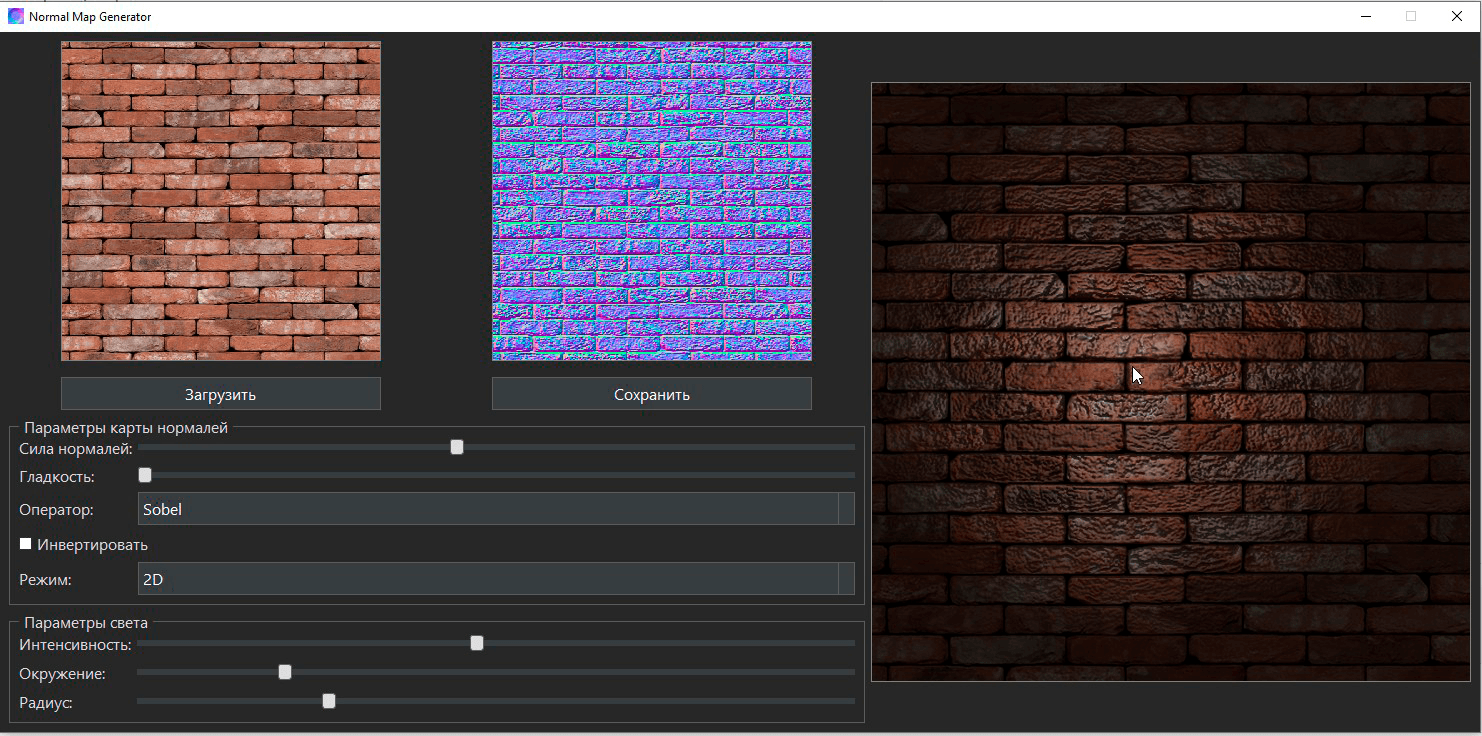
\includegraphics[width=1\linewidth]{testsave}}
	\caption{Загрузка изображения}
	\label{testsave:image}
\end{figure}

\subsubsection{Загрузка неподдерживаемого файла}

Сценарий: пользователь выбирает файл с неподдерживаемым расширением, например .txt или .mp3.

Ожидаемый результат: программа сообщает о невозможности загрузки изображения. Интерфейс остаётся стабильным.

Фактический результат: выведено сообщение об ошибке, работа программы не прерывается.

Результат системного тестирования представлен на рисунке \ref{testnoimage:image}.

\begin{figure}[H]
	\center{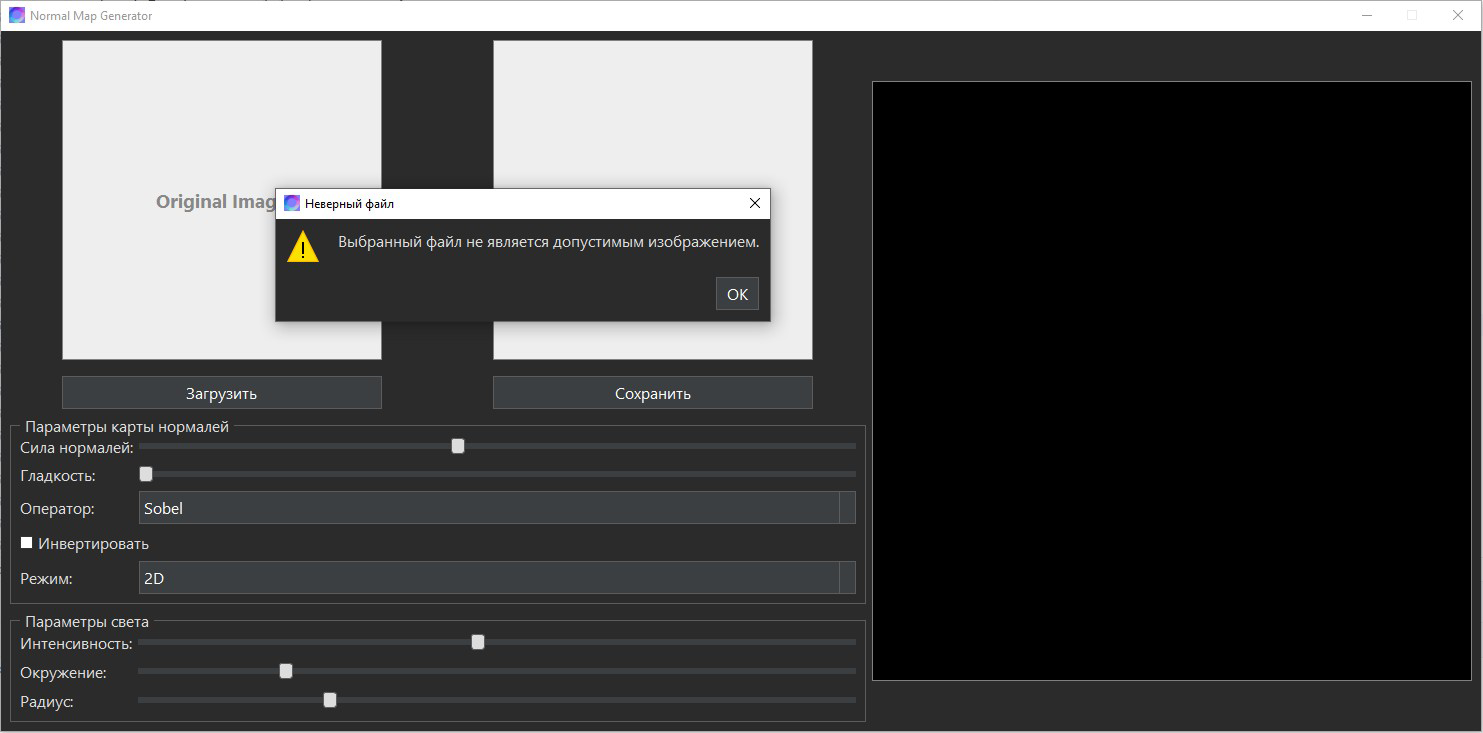
\includegraphics[width=1\linewidth]{testnoimage}}
	\caption{Загрузка неподдерживаемого файла}
	\label{testnoimage:image}
\end{figure}

\subsubsection{Изменение параметров генерации}

Сценарий: пользователь изменяет значение ползунка «Сила нормалей» и «Гладкость», переключает оператор градиента.

Ожидаемый результат: карта нормалей в окне визуализации обновляется в реальном времени при любом изменении параметров.

Фактический результат: визуализация обновляется мгновенно. Все изменения корректно отражаются на результатах.
\newpage
Результат системного тестирования представлен на рисунке \ref{testupstr:image}.

\begin{figure}[H]
	\center{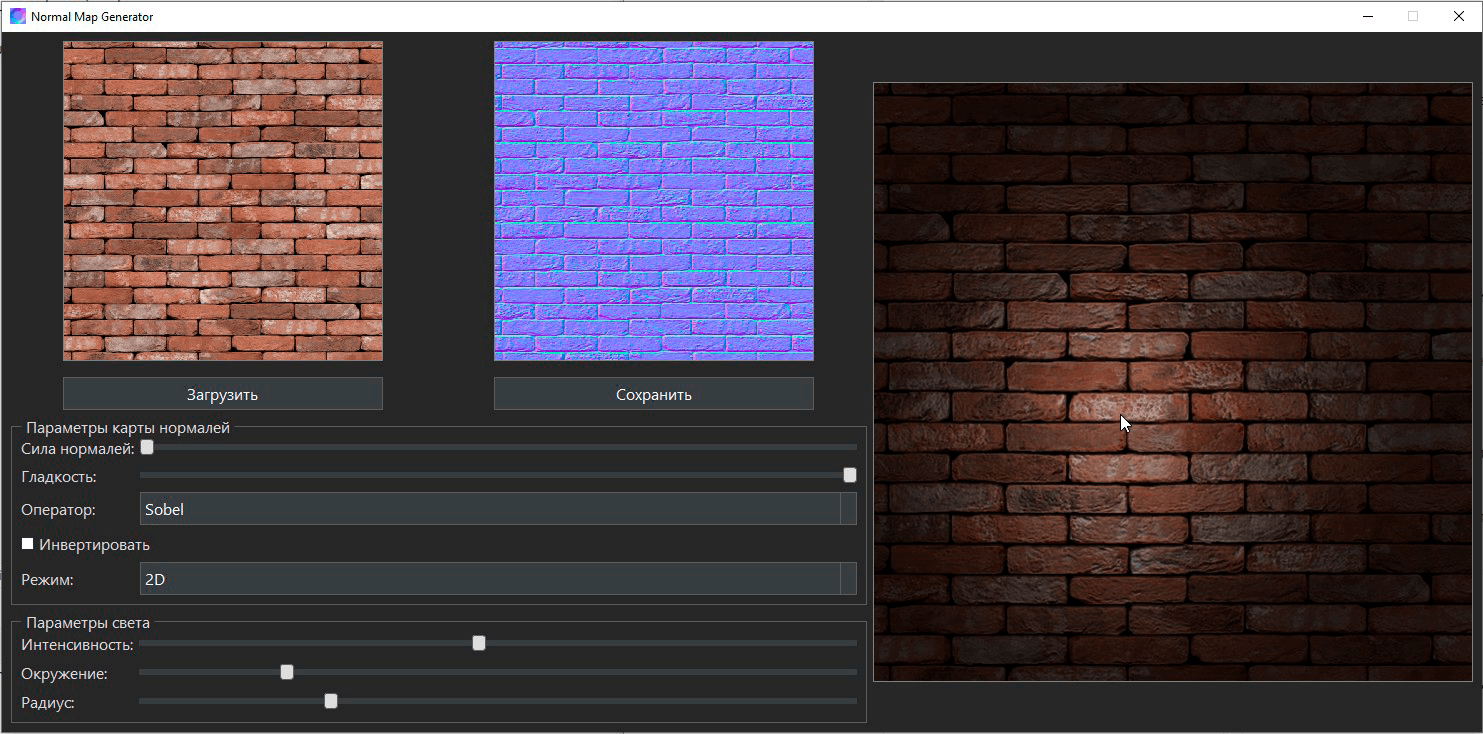
\includegraphics[width=1\linewidth]{testupstr}}
	\caption{Изменение параметров генерации}
	\label{testupstr:image}
\end{figure}

\subsubsection{Сохранение карты нормалей}

Сценарий: пользователь нажимает кнопку «Сохранить» и выбирает путь на диске.

Ожидаемый результат: файл с изображением карты нормалей сохраняется по указанному пути.

Фактический результат: изображение сохраняется корректно, без потери качества.
\newpage
Результат системного тестирования представлен на рисунке \ref{testsavenm:image}.

\begin{figure}[H]
	\center{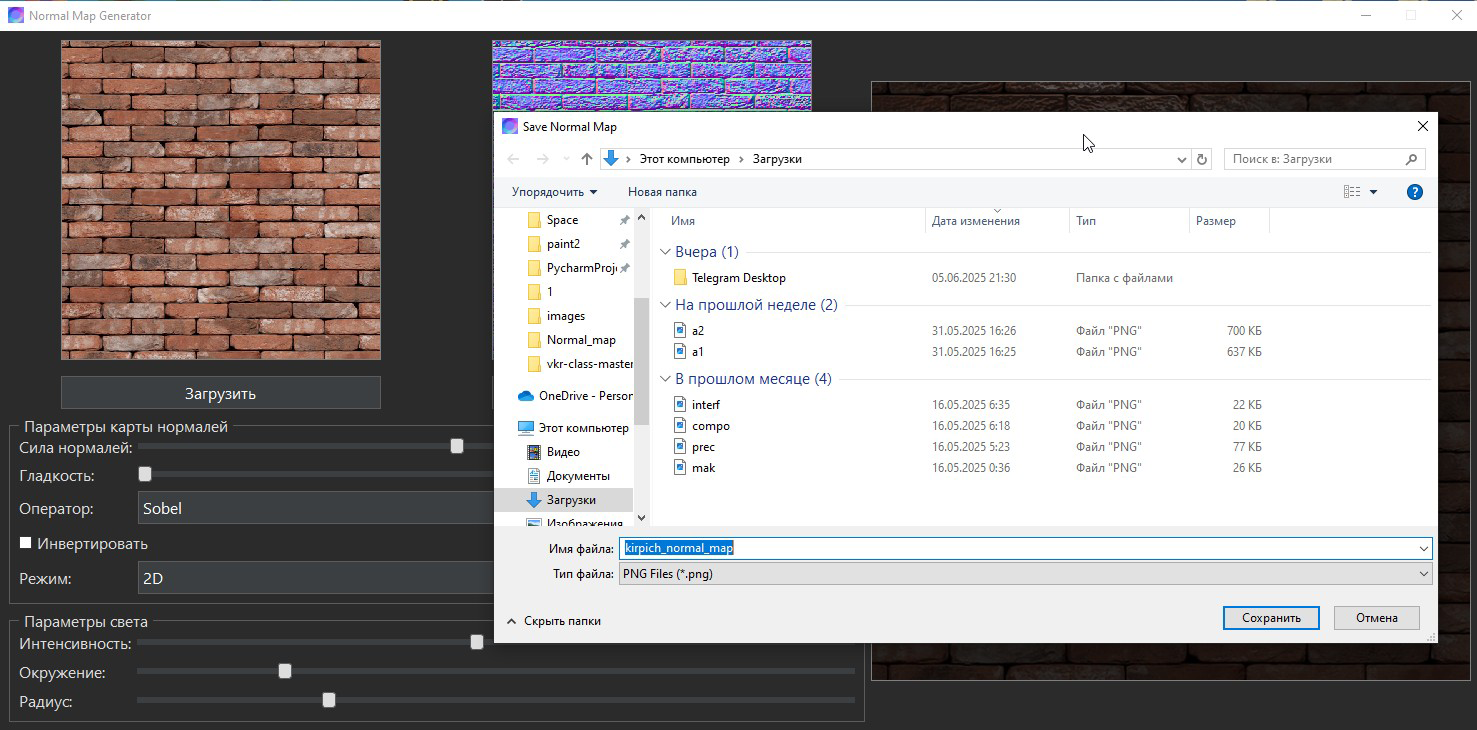
\includegraphics[width=1\linewidth]{testsavenm}}
	\caption{Сохранение карты нормалей}
	\label{testsavenm:image}
\end{figure}

\subsubsection{Изменение параметров света}

Сценарий: пользователь изменяет значение ползунка «Интенсивность», «Окружение» и «Радиус».

Ожидаемый результат: карта нормалей в окне визуализации обновляется в соответствии с новыми параметрами света.

Фактический результат: визуализация обновляется мгновенно. Все изменения корректно отражаются на результатах.
\newpage
Результат системного тестирования представлен на рисунке \ref{testint:image}.

\begin{figure}[H]
	\center{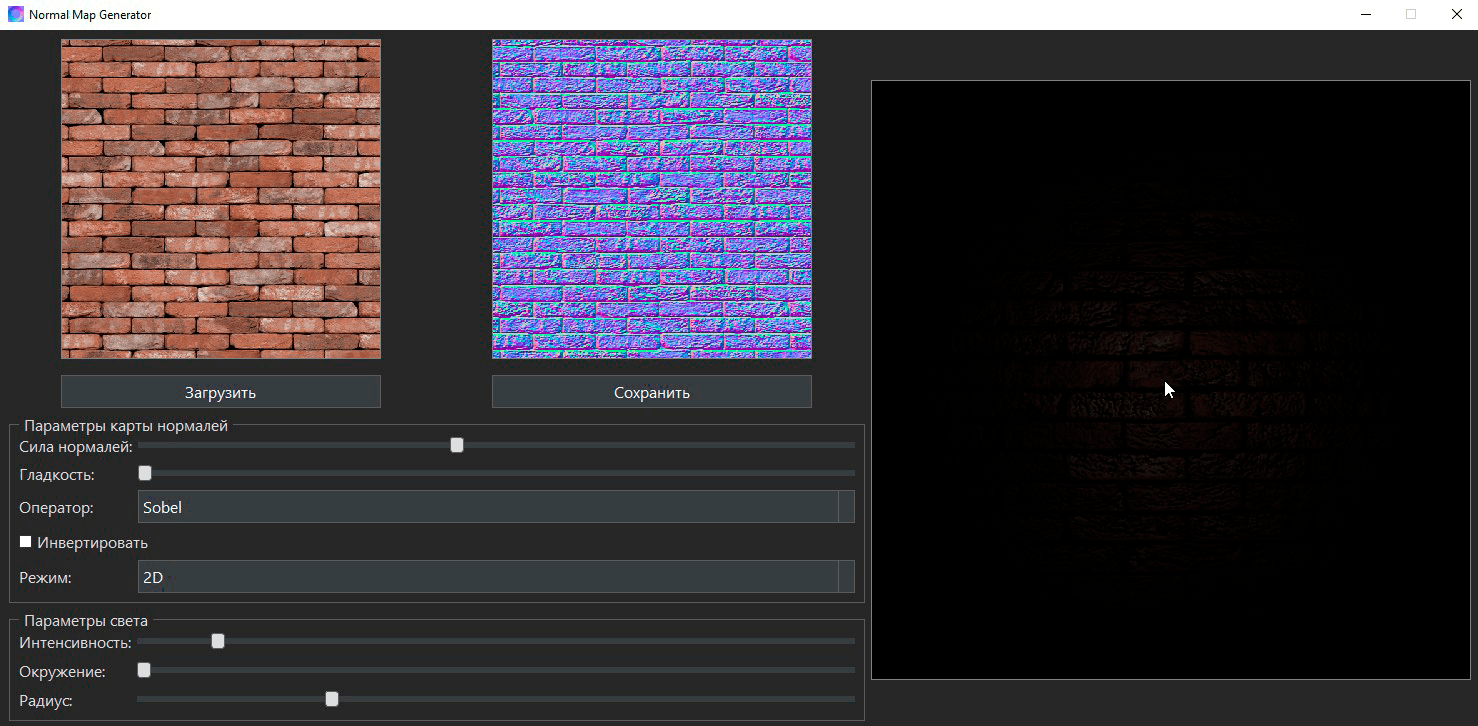
\includegraphics[width=1\linewidth]{testint}}
	\caption{Изменение параметров света}
	\label{testint:image}
\end{figure}

\subsubsection{Работа 3D-режима визуализации}

Сценарий: пользователь выбирает в выпадающем списке режим «3D». Отображается куб с наложенным изображением и освещением. Пользователь вращает куб, используя мышь.

Ожидаемый результат: куб вращается, направление света остаётся постоянным, тени на поверхностях меняются в зависимости от нормалей. Все грани текстурированы корректно.

Фактический результат: 3D-визуализация работает плавно. При перемещении мыши куб вращается без задержек. Световое пятно перемещается согласно направлению нормалей.
\newpage
Результат системного тестирования представлен на рисунке \ref{test3d:image}.

\begin{figure}[H]
	\center{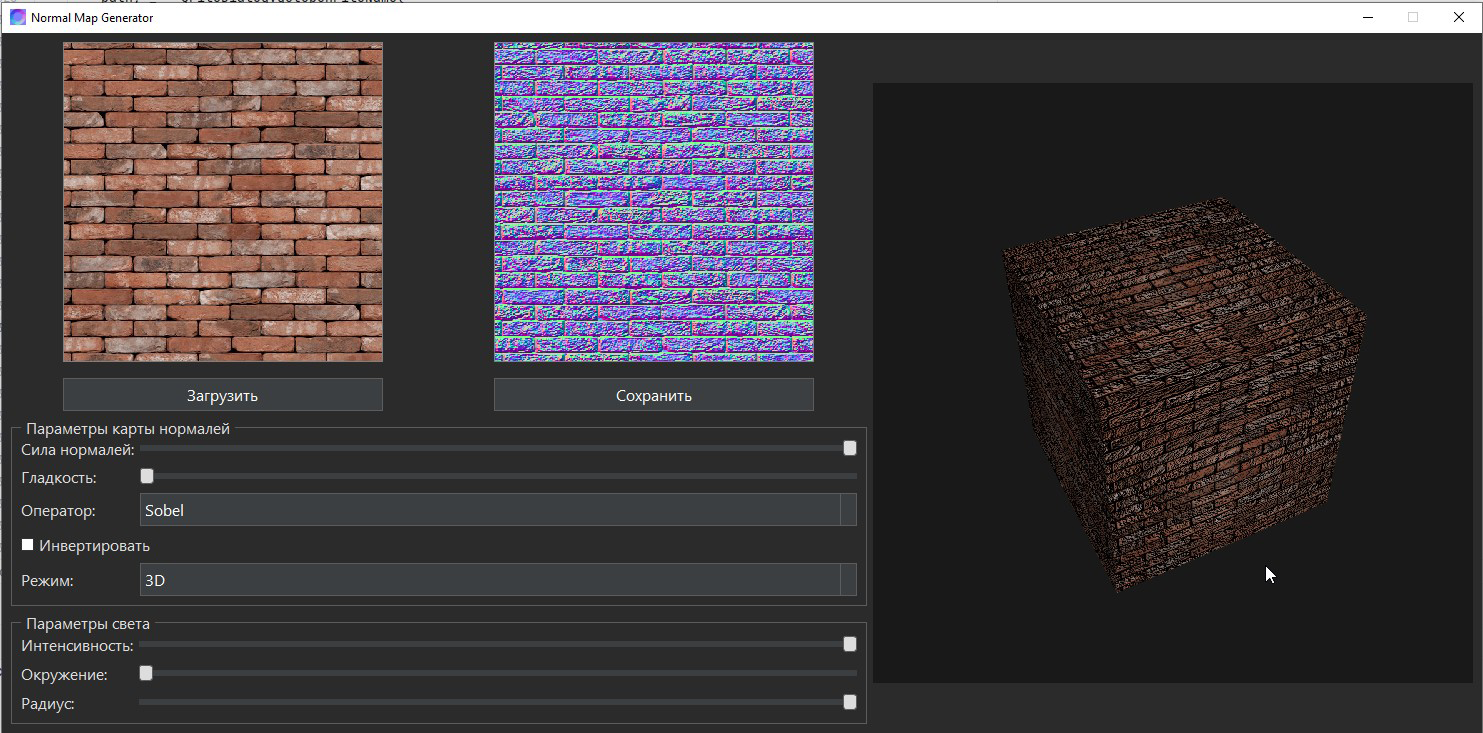
\includegraphics[width=1\linewidth]{test3d}}
	\caption{Работа 3D-режима визуализации}
	\label{test3d:image}
\end{figure}

\subsubsection{Быстрое переключение между 2D и 3D режимами}

Сценарий: пользователь быстро переключается между режимами отображения.

Ожидаемый результат: переключение проходит корректно, программа не зависает и не теряет данные.

Фактический результат: режимы переключаются без ошибок. Все параметры сохраняются при переходе между режимами.
\newpage
Результат системного тестирования представлен на рисунке \ref{testswap:image}.

\begin{figure}[H]
	\center{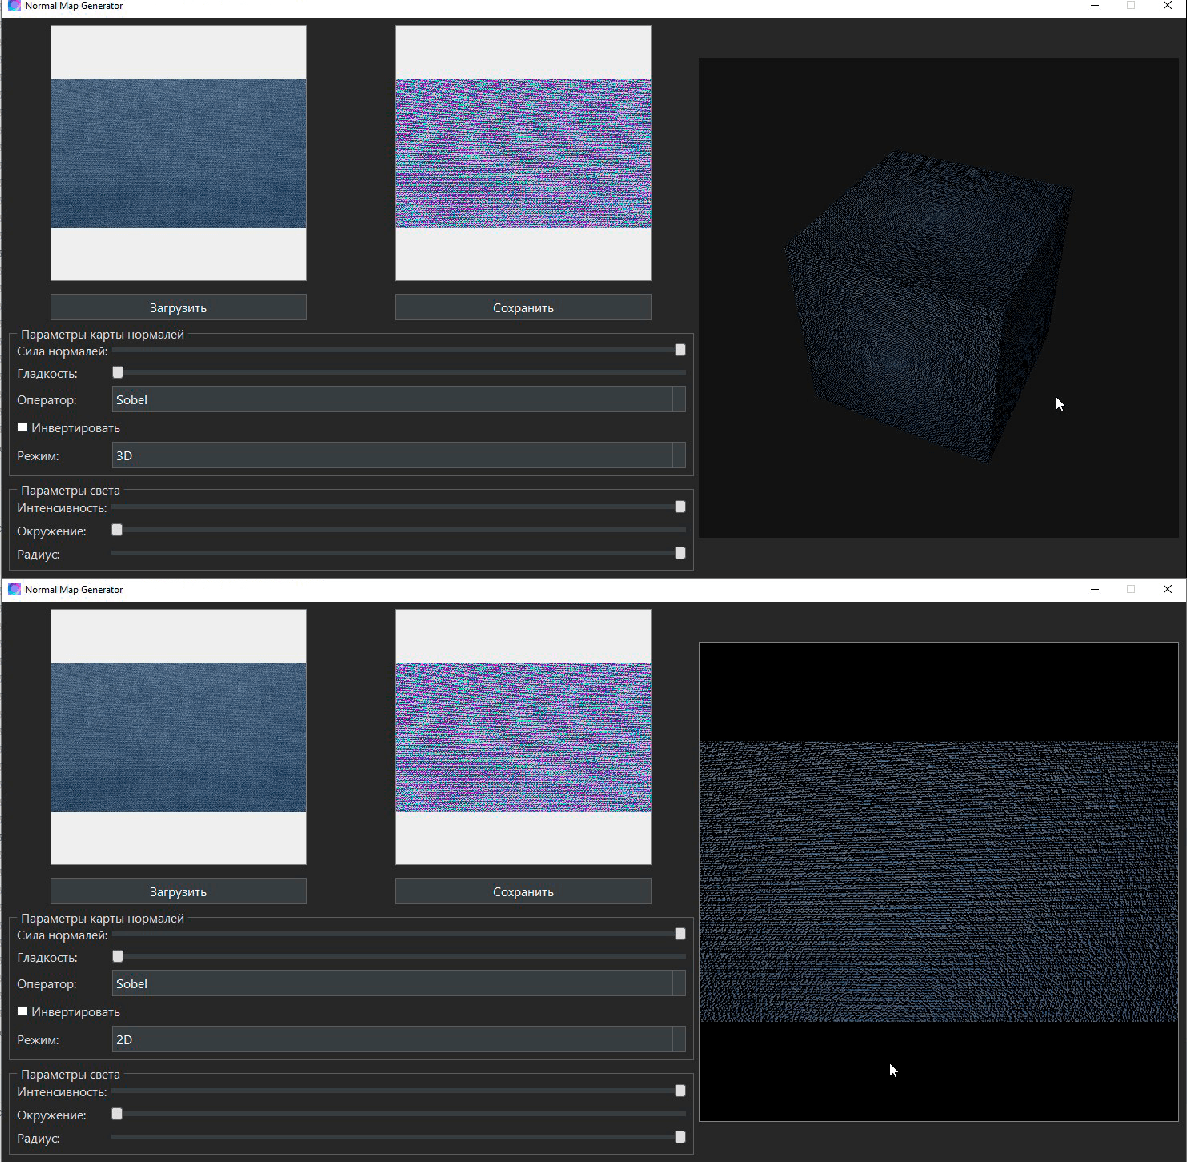
\includegraphics[width=1\linewidth]{testswap}}
	\caption{Быстрое переключение между 2D и 3D режимами}
	\label{testswap:image}
\end{figure}

\subsubsection{Обработка изображения с высоким разрешением}

Сценарий: пользователь загружает изображение высокого разрешения (например, 4096×4096 пикселей).

Ожидаемый результат: программа не принимает изображение, если его разрешение больше 2048×2048. Пользователь получает предупреждение.

Фактический результат: программа не обработала изображение. Появляется предупреждение с информацией о допустимых размерах.
\newpage
Результат системного тестирования представлен на рисунке \ref{testbig:image}.

\begin{figure}[H]
	\center{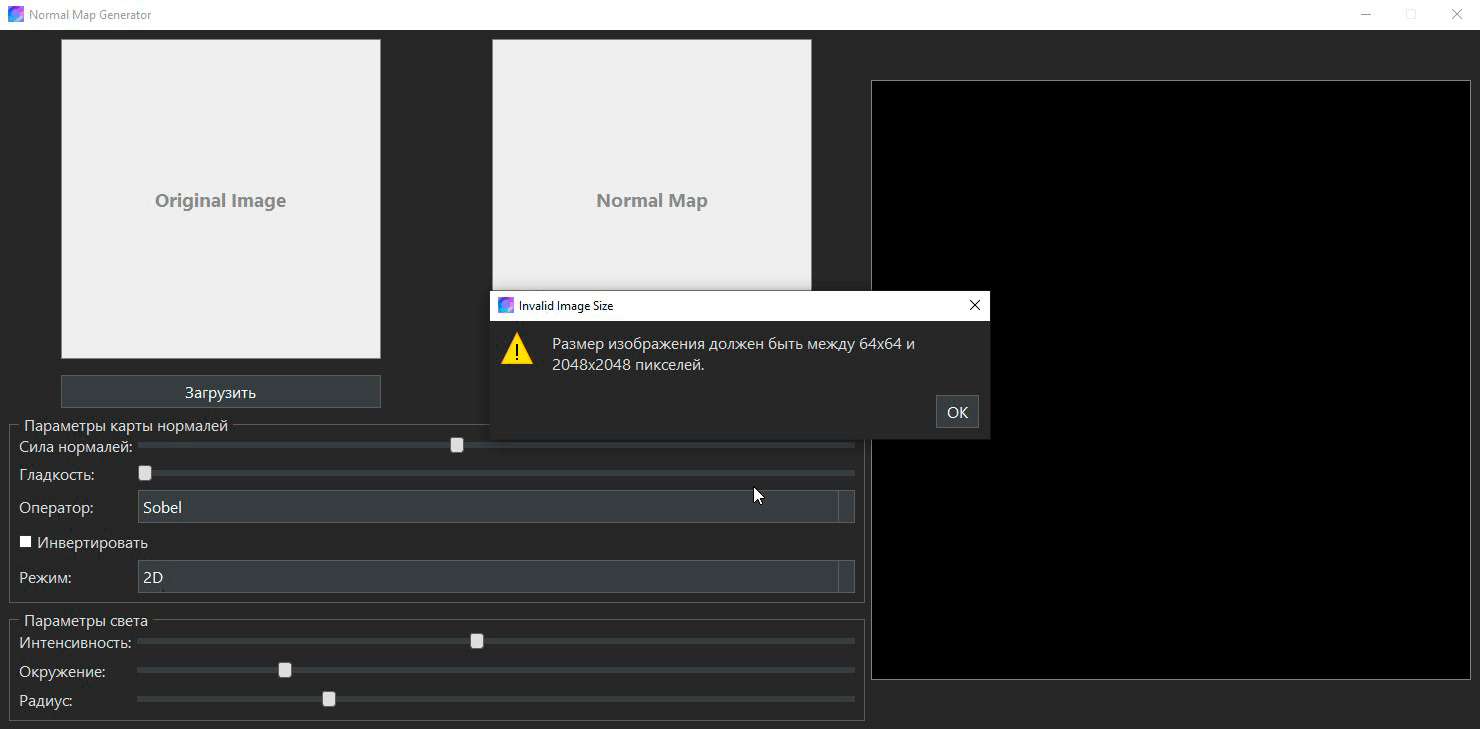
\includegraphics[width=1\linewidth]{testbig}}
	\caption{Обработка изображения с высоким разрешением}
	\label{testbig:image}
\end{figure}

\subsubsection{Инверсия карты нормалей}

Сценарий: пользователь активирует чекбокс «Инвертировать нормали».

Ожидаемый результат: отображение карты нормалей и визуализация освещения изменяются соответствующим образом — направления нормалей инвертируются.

Фактический результат: результат изменяется корректно, визуально ощущается изменение направления света на изображении.
\newpage
Результат системного тестирования представлен на рисунке \ref{testinv:image}.

\begin{figure}[H]
	\center{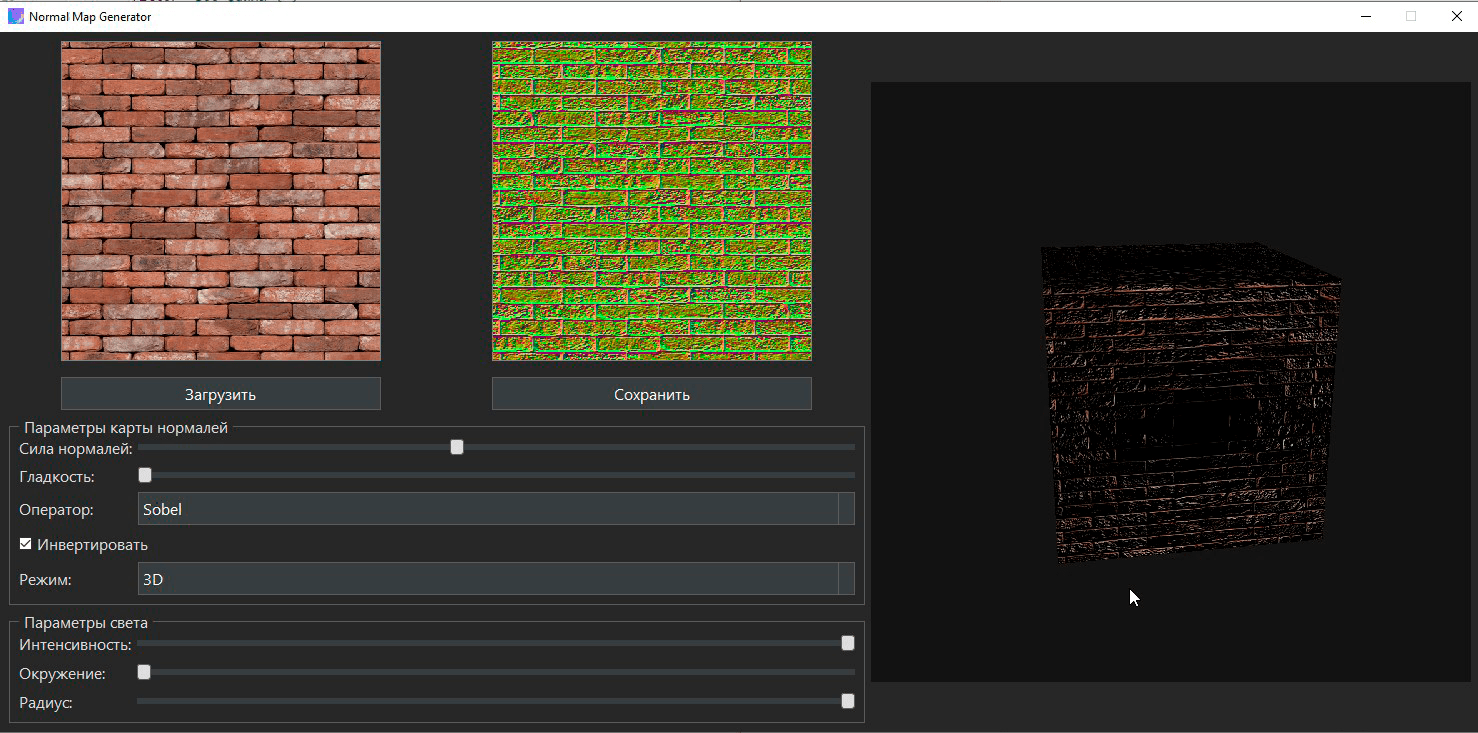
\includegraphics[width=1\linewidth]{testinv}}
	\caption{Инверсия карты нормалей}
	\label{testinv:image}
\end{figure}

\subsubsection{Перемещение источника света в режиме 2D}

Сценарий: пользователь перемещает курсор мыши по области визуализации в 2D-режиме.

Ожидаемый результат: освещение на изображении изменяется в соответствии с положением мыши — «фонарик» движется, создавая эффект направления света.

Фактический результат: реакция на перемещение мыши плавная, освещение обновляется в реальном времени.
\newpage
Результат системного тестирования представлен на рисунке \ref{testfon:image}.

\begin{figure}[H]
	\center{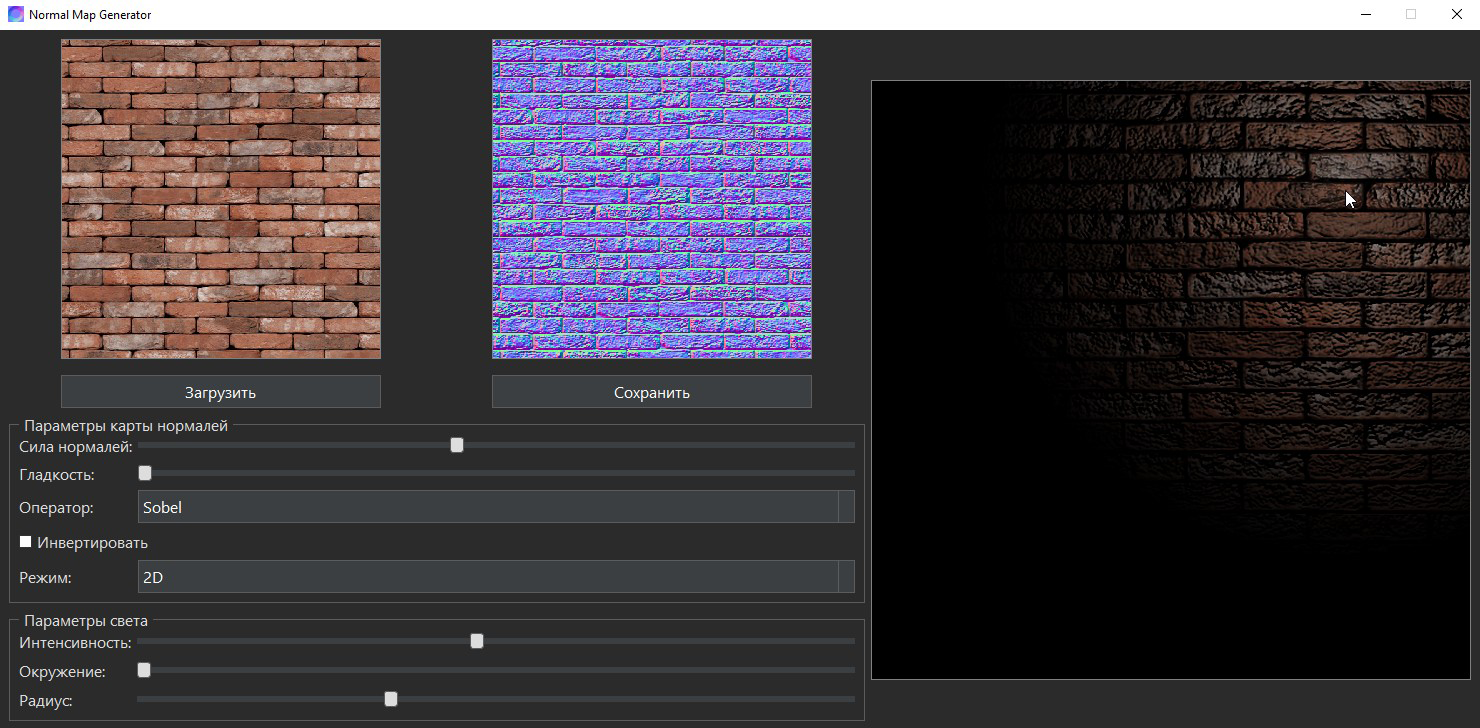
\includegraphics[width=1\linewidth]{testfon}}
	\caption{Перемещение источника света в режиме 2D}
	\label{testfon:image}
\end{figure}

\begin{comment}
На рисунке \ref{main:image} представлена главная страница сайта «Русатом – Аддитивные технологии».
\newpage % при необходимости можно переносить рисунок на новую страницу
\begin{figure}[H] % H - рисунок обязательно здесь, или переносится, оставляя пустоту
\center{\includegraphics[width=1\linewidth]{main1}}
\center{\includegraphics[width=1\linewidth]{main2}}
\center{\includegraphics[width=1\linewidth]{main3}}
\caption{Главная страница сайта «Русатом – Аддитивные технологии»}
\label{main:image}
\end{figure}

На рисунке \ref{menu:image} представлен динамический вывод заголовков, включающий в себя искомые фразы при поиске фраз.

\begin{figure}[ht]
\center{\includegraphics[width=1\linewidth]{menu}}
\caption{Динамический вывод заголовков}
\label{menu:image}
\end{figure}

На рисунке \ref{enter:image} представлен ввод данных для публикации новости.

\begin{figure}[ht]
\center{\includegraphics[width=1\linewidth]{enter}}
\caption{Ввод данных для публикации очень-очень длинной, интересной и полезной новости}
\label{enter:image}
\end{figure}
\end{comment}